\documentclass[handout]{beamer} % Use the beamer class for presentations, 'handout' option to suppress \pause

\input{Lecture-Slides/preamble.txt}

% Define the transition slide command
\newcommand{\transitionslide}[1]{
    \begin{frame} %%%%%%%%%%%%%%%%%%%%%%%%%%%%%%%%%%%%%%%%%%%%%%%%%%%%%%%%%%[plain]
        \centering
        \vspace{1cm}
        \Huge
        \textcolor{moonstoneblue!150}{\textbf{#1}}
    \end{frame}
}

% Title and Author Info
\title{Introduction to Statistical Methods in Political Science}
\subtitle{Lecture 6: Expected Value and Population Parameters}
\author{Ignacio Urbina \texorpdfstring{\\ \vspace{0.3em}}{ } \scriptsize \textcolor{gray}{Ph.D. Candidate in Political Science}}
\date{}

%%%%%%%%%%%%%%%%%%%%%%%%%%%%%%%%%%%%%%%%%%%%%%%%%%%%%%%%%%%%%%%%%%%%%%%%%%%%%%
%%% DATA

%%%%%%%%%%%%%%%%%%%%%%%%%%%%%%%%%%%%%%%%%%%%%%%%%%%%%%%%%%%%%%%%%%%%%%%%%%
%%% BEGIN DOC

\begin{document}
\frame{\titlepage}

%%%%%%%%%%%%%%%%%%%%%%%%%%%%%%%%%%%%%%%%%%%%%%%%%%%%%%%%%%%%%%%%%%%%%%%%%%
\section{Random Variables and their Probability Distributions}

\transitionslide{Population Parameters and the Expected Value}

%%%%%%%%%%%%%%%%%%%%%%%%%%%%%%%%%%%%%%%%%%%%%%%%%%%%%%%%%%%%%%%%%%%%%%%%%%%%%%
\begin{frame} %%%%%%%%%%%%%%%%%%%%%%%%%%%%%%%%%%%%%%%%%%%%%%%%%%%%%%%%%%
\frametitle{Introduction to Population Parameters}

\begin{itemize}
  \item Population parameters (e.g., $\mu_X$ and $\sigma_X^2$) are numeric, deterministic values that summarize the characteristics of a population's distribution.
  \pause
  \item These parameters include measurements of central tendency and spread (i.e., dispersion), providing insights into the general behavior and variability of the population.
  \pause
  \item Population parameters are not random variables themselves; they are fixed quantities calculated from the distribution of a random variable.
\end{itemize}

\end{frame}

%%%%%%%%%%%%%%%%%%%%%%%%%%%%%%%%%%%%%%%%%%%%%%%%%%%%%%%%%%%%%%%%%%%%%%%%%%%%%%
\begin{frame} %%%%%%%%%%%%%%%%%%%%%%%%%%%%%%%%%%%%%%%%%%%%%%%%%%%%%%%%%%
\frametitle{Expectation: The Expected Value of a Random Variable}

\begin{itemize}
  \item What is the \textbf{expected value} or \textbf{expectation} of a random variable?
  \pause
  \item Simply put, the expected value is the \textbf{center} of the distribution.
  \pause
  \item But what do we mean by \textbf{center}?
  \pause
  \begin{itemize}
    \item It is the point that balances the distribution’s domain in a precise mathematical sense.
  \end{itemize}
  \pause
  \item More formally, the expected value of $X$ is the point where its distribution’s \textbf{center of mass} lies, balancing the weighted distances to all other points.
  \pause
  \item Thus, the \textbf{expectation} of $X$, written as $E[X]$, equals its \textbf{population mean}:
    \[
    E[X] = \mu_X.
    \]
\end{itemize}

\end{frame}

%%%%%%%%%%%%%%%%%%%%%%%%%%%%%%%%%%%%%%%%%%%%%%%%%%%%%%%%%%%%%%%%%%%%%%%%%%%%%%
\begin{frame} %%%%%%%%%%%%%%%%%%%%%%%%%%%%%%%%%%%%%%%%%%%%%%%%%%%%%%%%%%
\frametitle{Formal Definition of \(E(X)\) - Discrete RV}

\begin{itemize}
  \item Let $X$ be some \textbf{discrete random variable (RV)}.
  \item The \emph{Expected Value} of $X$ is defined as:
  \pause
  \[
  E(X) = \sum_{x \in D_X} x \cdot p_X(x)
  \]
  \pause
  \item Here, \(p_X(x)\) is the probability mass function (PMF) of \(X\).
  \pause
  \item $D_X$ is the domain of $X$, that is, all the values $X$ can take.
  \pause
  \item Note that $E(X)$, at any given point in time, is an unknown constant, not a random variable.
\end{itemize}

\end{frame}

\begin{frame} %%%%%%%%%%%%%%%%%%%%%%%%%%%%%%%%%%%%%%%%%%%%%%%%%%%%%%%%%% %%%%%%%%%%%%%%%%%%%%%%%%%%%%%%%%%%%%%%%%%%%%%%%%%%%%%
\frametitle{Graphical Example: Symmetric Distribution}
\vspace{1.5em}

\begin{figure}[ht]
\centering
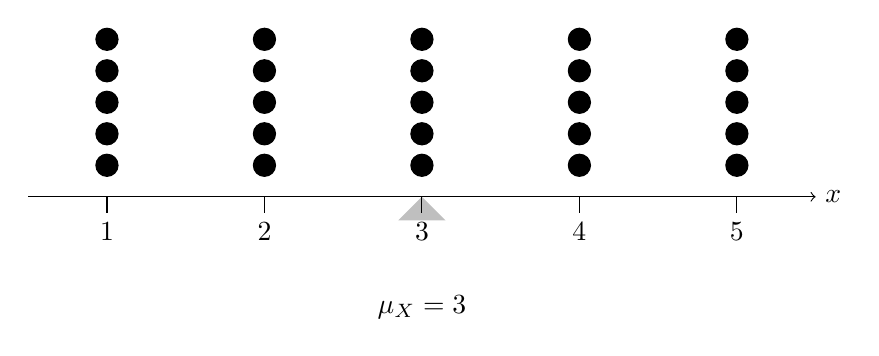
\begin{tikzpicture}[scale=2]
  % Dots for symmetric distribution
  \foreach \x in {1, 2, 3, 4, 5} {
    \foreach \y in {1, 2, 3, 4, 5} {
      \filldraw (\x, \y*0.2) circle (2pt);
    }
  }

  % Shaded triangle below the mean value (x=3)
  \fill[gray, opacity=0.5] (2.85, -0.15) -- (3, 0) -- (3.15, -0.15) -- cycle;

  % X-axis
  \draw[->] (0.5, 0) -- (5.5, 0) node[right] {$x$};
  \foreach \x in {1, 2, 3, 4, 5} {
    \draw (\x, 0) -- (\x, -0.1) node[below] {\x};
  }

  % Labels
  \node at (3, -0.7) {$\mu_X = 3$};

\end{tikzpicture}
\end{figure}

\end{frame}

%%%%%%%%%%%%%%%%%%%%%%%%%%%%%%%%%%%%%%%%%%%%%%%%%%%%%%%%%%%%%%%%%%%%%%%%%%%%%%
\begin{frame} %%%%%%%%%%%%%%%%%%%%%%%%%%%%%%%%%%%%%%%%%%%%%%%%%%%%%%%%%%
\frametitle{Graphical Example: Symmetric Distribution}
\vspace{1.5em}
  \pause

\begin{figure}[ht]
\centering
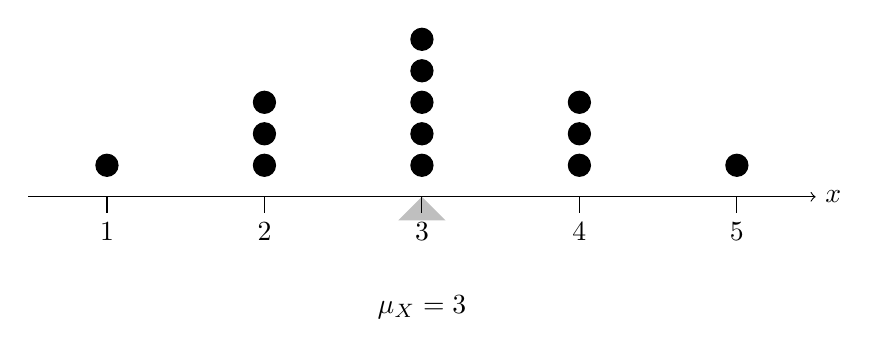
\begin{tikzpicture}[scale=2]
  % Dots for symmetric distribution
    \foreach \y in {1} {
      \filldraw (1, \y*0.2) circle (2pt);
      \filldraw (5, \y*0.2) circle (2pt);
    }
    \foreach \y in {1,2,3} {
      \filldraw (2, \y*0.2) circle (2pt);
      \filldraw (4, \y*0.2) circle (2pt);
    }
    \foreach \y in {1,2,3,4,5} {
      \filldraw (3, \y*0.2) circle (2pt);
    }

  % Shaded triangle below the mean value (x=3)
  \fill[gray, opacity=0.5] (2.85, -0.15) -- (3, 0) -- (3.15, -0.15) -- cycle;

  % X-axis
  \draw[->] (0.5, 0) -- (5.5, 0) node[right] {$x$};
  \foreach \x in {1, 2, 3, 4, 5} {
    \draw (\x, 0) -- (\x, -0.1) node[below] {\x};
  }

  % Labels
  \node at (3, -0.7) {$\mu_X = 3$};

\end{tikzpicture}
\end{figure}

\end{frame}

%%%%%%%%%%%%%%%%%%%%%
\begin{frame} %%%%%%%%%%%%%%%%%%%%%%%%%%%%%%%%%%%%%%%%%%%%%%%%%%%%%%%%%%
\frametitle{Graphical Example: Skewed Distribution}
\vspace{1.5em}
  \pause

\begin{figure}[ht]
\centering
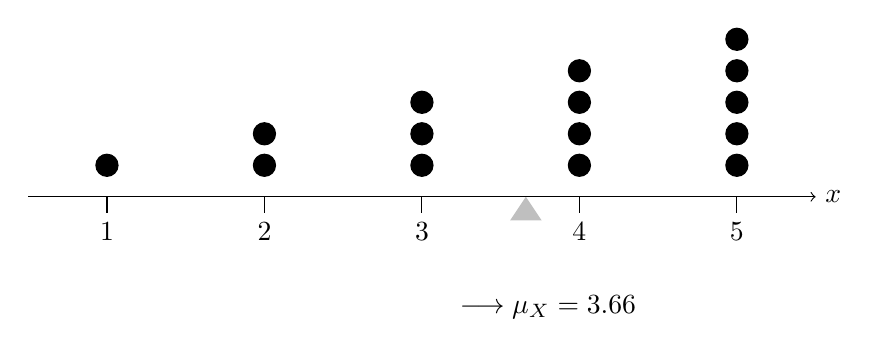
\begin{tikzpicture}[scale=2]
  % Dots for asymmetric distribution
  \foreach \x in {1, 2, 3, 4, 5} {
    \pgfmathsetmacro{\ymax}{\x} % Set ymax as the value of x
    \foreach \y in {1, ..., \ymax} {
      \filldraw (\x, \y*0.2) circle (2pt);
    }
  }

  % Shaded triangle below the mean value (x=3.66)
  \fill[gray, opacity=0.5] (3.56, -0.15) -- (3.66, 0) -- (3.76, -0.15) -- cycle;

  % X-axis
  \draw[->] (0.5, 0) -- (5.5, 0) node[right] {$x$};
  \foreach \x in {1, 2, 3, 4, 5} {
    \draw (\x, 0) -- (\x, -0.1) node[below] {\x};
  }

  % Labels
  \node at (3.80, -0.7) {$\longrightarrow \mu_X = 3.66$};

\end{tikzpicture}
\end{figure}

\end{frame}

\begin{frame} %%%%%%%%%%%%%%%%%%%%%%%%%%%%%%%%%%%%%%%%%%%%%%%%%%%%%%%%%%
\frametitle{Formal Definition of \(E(X)\) - Continous RV}

\begin{itemize}
  \item Let $X$ be a \textbf{continuous random variable}.
  \item The expected value of $X$ is defined as:
  \pause
  \[
  E(X) = \int_{-\infty}^{\infty} x \cdot f_X(x) \, dx
  \]
  \pause
  \item \(f_X(x)\) is the probability density function (PDF) of \(X\).
  \pause
  \item The integral captures the total weighted area, just like a sum does in the discrete case.
  \pause
  \item Just as a sum adds up discrete contributions, the integral accumulates contributions over a continuous range.
\end{itemize}

\end{frame}


\begin{frame} %%%%%%%%%%%%%%%%%%%%%%%%%%%%%%%%%%%%%%%%%%%%%%%%%%%%%%%%%%
    \frametitle{Conceptual Illustration of $E(X)$ - Discrete RV}

    \begin{figure}
        \centering
        \makebox[\textwidth]{ % Expands the box to the full width
            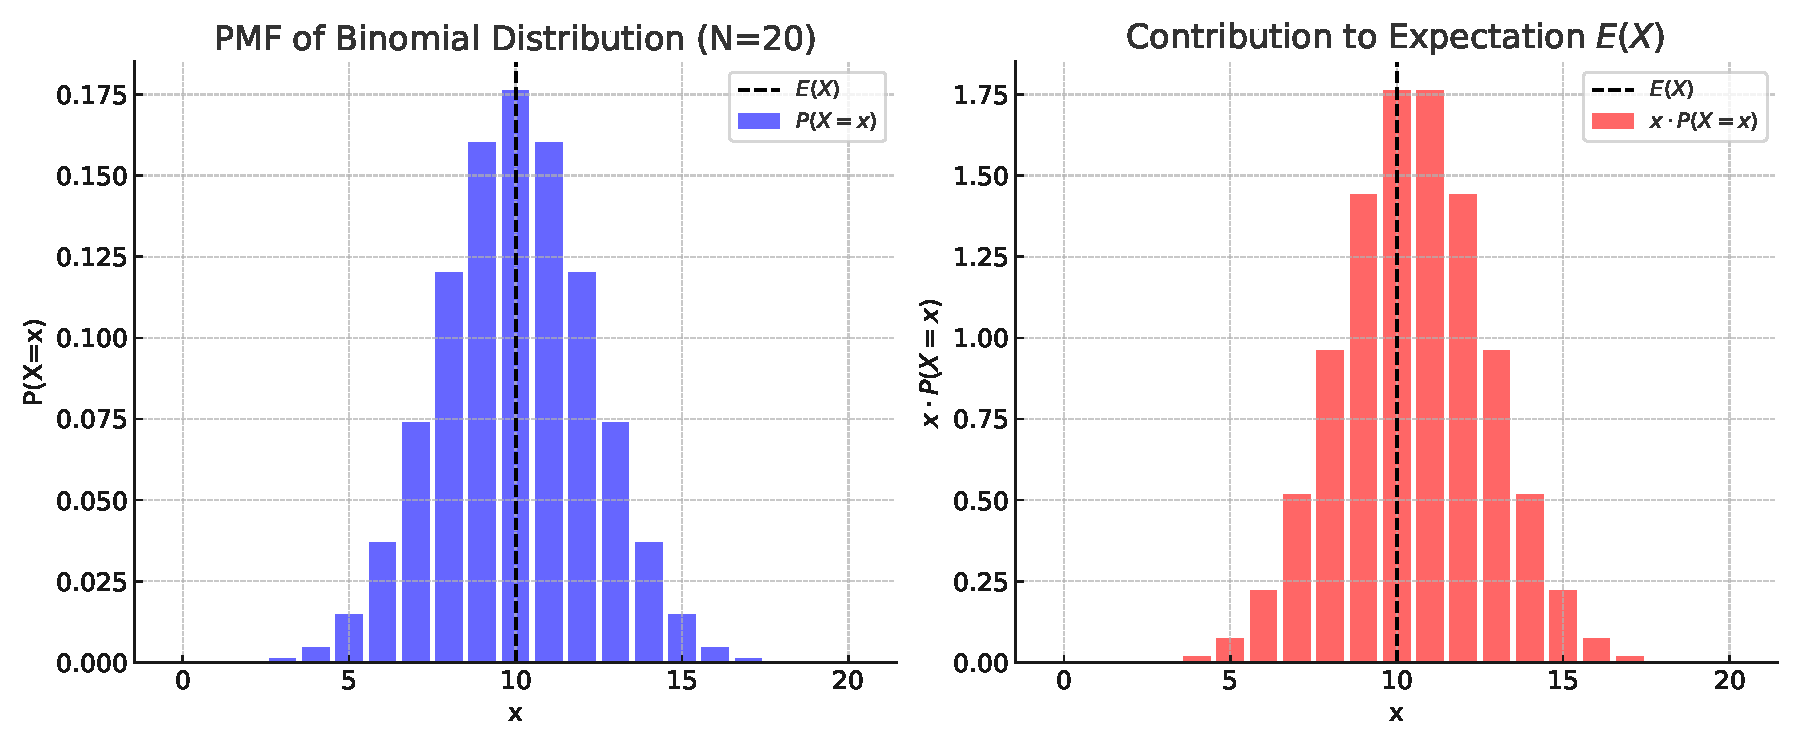
\includegraphics[width=1.15\textwidth]{Figures/binomial_distribution.pdf}
        }
    \end{figure}

\end{frame}

\begin{frame} %%%%%%%%%%%%%%%%%%%%%%%%%%%%%%%%%%%%%%%%%%%%%%%%%%%%%%%%%%
    \frametitle{Conceptual Illustration of $E(X)$ - Continuous RV}

    \begin{figure}
        \centering
        \makebox[\textwidth]{ % Expands the box to the full width
            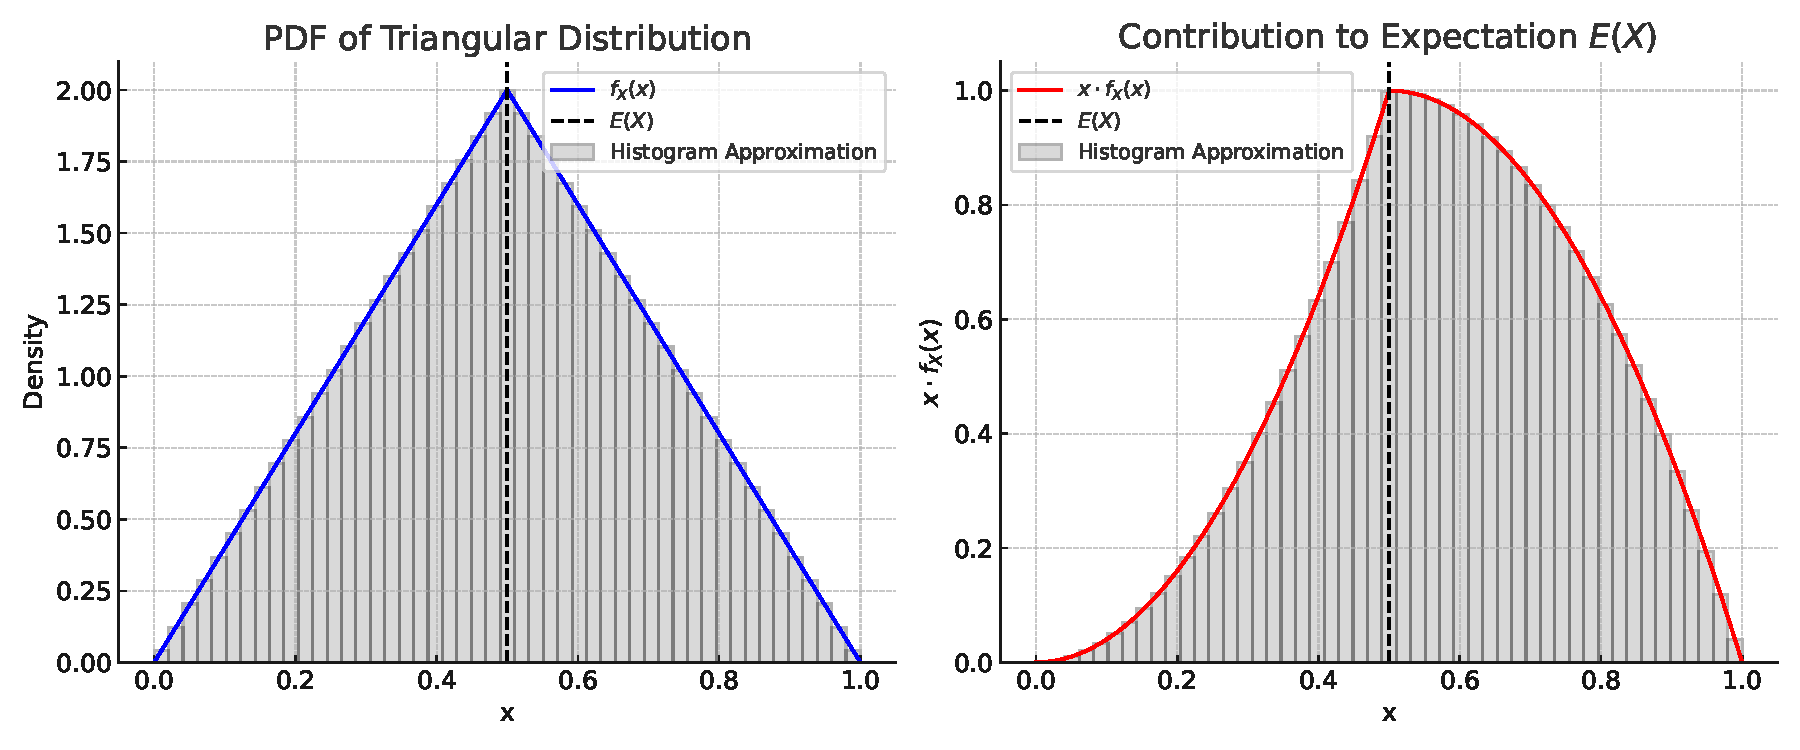
\includegraphics[width=1.15\textwidth]{Figures/triangular_distribution.pdf}
        }
    \end{figure}

\end{frame}

\begin{frame} %%%%%%%%%%%%%%%%%%%%%%%%%%%%%%%%%%%%%%%%%%%%%%%%%%%%%%%%%%
\frametitle{Example: Discrete RV Representing Ideology}

\begin{minipage}{0.45\textwidth}
    \textbf{PMF Table:}
    \begin{table}[h]
        \centering
        \begin{tabular}{c|c}
        \textbf{x (Ideology)} & $\bm{P(X=x)}$ \\
        \hline
        -5 \text{ (Far left) } & 0.05 \\
        -4 & 0.10 \\
        -3 & 0.15 \\
        -2 & 0.20 \\
        -1 & 0.20 \\
         0 & 0.10 \\
         1 & 0.10 \\
         2 & 0.05 \\
         3 & 0.03 \\
         4 & 0.02 \\
         5 \text{ (Far right) } & 0.00 \\
        \end{tabular}
    \end{table}
  \pause
\end{minipage}
        \hfill
\begin{minipage}{0.50\textwidth}
    \textbf{Expectation:}
    \begin{itemize}
        \pause
        \item Definition:
        \[
        E(X) = \sum_{\text{For all } x} x \cdot p_X(x)
        \]
        \pause
        \item Calculation:
    \end{itemize}
  \pause
    \vspace{0.2em}
        \small $$E(X) = (-5)(0.05) + (-4)(0.10) $$
        \pause
        \small $$\quad +(-3)(0.15) + (-2)(0.20) + (-1)(0.20)$$
        \pause
        \small $$\quad + (0)(0.10) + (1)(0.10) + (2)(0.05)$$
        \pause
        \small $$\quad + (3)(0.03) + (4)(0.02) + (5)(0.00).$$
    \vspace{-1.2em}
  \pause
    \begin{itemize}
        \item Result: $E[X] = -1.33$
    \end{itemize}
\end{minipage}

\end{frame}


\begin{frame} %%%%%%%%%%%%%%%%%%%%%%%%%%%%%%%%%%%%%%%%%%%%%%%%%%%%%%%%%%
\frametitle{Some Remarks on Expectation}

\begin{itemize}
  \item Expectation allows us to define fundamental features of the true (unobserved) distribution of a random variable.
  \pause
  \item These features are always \textbf{centered} by the weights imposed by the probability distribution of the random variable.
  \pause
  \item As statistical analysts, our goal is to use samples to estimate these fundamental features, also called \textbf{population parameters}.
  \pause
  \item This process forms the foundation of statistical inference, enabling us to draw conclusions about the true distribution from observed data.
\end{itemize}

\end{frame}

\begin{frame} %%%%%%%%%%%%%%%%%%%%%%%%%%%%%%%%%%%%%%%%%%%%%%%%%%%%%%%%%%
\frametitle{Population Variance Expressed Using Expectations}

\begin{itemize}
  \item Analogously to the population mean, we can express the population variance using expectations.
  \pause
  \item Population variance measures the \textbf{expected quadratic deviation from the population mean.}
  \pause
  \item Considering the population probability distribution, we ask: what is the expected quadratic deviation from the mean?
  \pause
  \item This approach helps us understand how much the values of a \emph{random variable deviate}, on average, from the mean.
\end{itemize}

\end{frame}

\begin{frame} %%%%%%%%%%%%%%%%%%%%%%%%%%%%%%%%%%%%%%%%%%%%%%%%%%%%%%%%%%
\frametitle{Population Variance: Formal Definition Using Expectation}
\begin{itemize}
  \item Formal Definition:
  \pause
  \begin{align*}
      V(X) = \sigma_X^2 &=  E[(X - E(X))^2]  \\
                        &=  E[(X - \mu_X)^2].
  \end{align*} \vspace{-1em}
  \pause
\item $V(X)$ and $\sigma_X^2$ are alternative notations for ``\emph{the variance of $X$}."   \pause
\item The population variance is a ``centered" measure of the squared deviation of $X$ from its population mean.    \pause
\begin{itemize}
    \item So, $\sigma_X^2$ is also an expected value! (only that we take expectation with regard to $(X - E(X))^2$ and not just $X$)
\end{itemize}

\end{itemize}
\end{frame}

\begin{frame}
\frametitle{Population Variance: Discrete Case}

\begin{itemize}
  \item Variance measures the expected squared deviation from the mean.
  \item For a discrete random variable:
  \[
  V(X) =  E[(X - \mu_X)^2] =  \sum_{x \in D_X} (x - \mu_X)^2 \cdot p_X(x)
  \]
  \item Where $\mu_X = E(X)$ is the expected value of $X$.
  \begin{itemize}
      \item \textbf{Note 1}: Population SD is given by $\sigma_X = \sqrt{V(X)} = \sqrt{E[(X-\mu)^2]} $
      \item \textbf{Note 2}: A general property of expectations is, given some function discrete RV, and any continuous function $g(x)$, then $E[g(x)] = \sum_{x \in D_X} g(x) \cdot p_X(x)$.
  \end{itemize}
\end{itemize}

\end{frame}

\begin{frame}
\frametitle{Population Variance: Continuous Case}

\begin{itemize}
  \item For a continuous random variable, variance is defined as:
  \[
  V(X) = E[(X - \mu_X)^2] = \int_{-\infty}^{\infty} (x - \mu_X)^2 \, \cdot f_X(x) \, dx
  \]
  \item Where $\mu_X = E(X)$ is the expected value of $X$, and $f_X(x)$ is the PDF of $X$.
\end{itemize}

\end{frame}


\begin{frame} %%%%%%%%%%%%%%%%%%%%%%%%%%%%%%%%%%%%%%%%%%%%%%%%%%%%%%%%%%
\frametitle{Population Mean, Variance, and SD for Common RVs Distributions}

\renewcommand{\arraystretch}{2.5} % Adjust this value to increase/decrease row height

\footnotesize
\centering
\begin{tabular}{|l|c|c|c|c|}
\hline
\textbf{Distrib.}  & \bm{$X$} & \bm{$E(X)$} & \bm{$ V(X)$} & \bm{$SD(X)=\sqrt{V(X)}$} \\
\hline
\pause Uniform & $X \sim U[a,b]$ & $\frac{a+b}{2}$ & $\frac{(b-a+1)^2 - 1}{12}$ & $\sqrt{\frac{(b-a+1)^2 - 1}{12}}$ \\
\hline
\pause Bernoulli & $X \sim Ber(p)$ & $p$ & $p(1-p)$ & $\sqrt{p(1-p)}$ \\
\hline
\pause Binomial & $X \sim Bin(n,p)$ & $np$ & $np(1-p)$ & $\sqrt{np(1-p)}$ \\
\hline
\pause Normal & $X \sim N(\mu, \sigma^2)$ & $\mu$ & $\sigma^2$ & $\sigma$ \\
\hline
\end{tabular}

\end{frame}

\begin{frame} %%%%%%%%%%%%%%%%%%%%%%%%%%%%%%%%%%%%%%%%%%%%%%%%%%%%%%%%%%
\frametitle{Example: Mean and Variance for Uniform Distribution (Die Roll)}

\begin{minipage}{0.45\textwidth}
\textbf{PMF for a Die Roll}
\begin{itemize}
    \item $p_X(x) = \frac{1}{6}$ for $x = 1, 2, 3, 4, 5, 6$
\end{itemize}
  \pause
\textbf{Population Mean:}
\begin{itemize}
    \pause
    \item  $E(X) = \mu = \sum_{i=1}^{6} (x_i) \cdot \frac{1}{6}$
    \pause
    \item[{}] $=\frac{1 + 2 + 3 + 4 + 5 + 6}{6} = \frac{21}{6} = 3.5.$
\end{itemize}
\end{minipage}
\hfill
\begin{minipage}{0.45\textwidth}
\textbf{Population Variance}
  \pause
\begin{itemize}
    \item $V(X) = \sigma^2 = E[(X-\mu)^2] =$
    \pause
    \item[{}] $ =\sum_{i=1}^{6} (x_i - \mu)^2 \cdot \frac{1}{6}$
    \pause
    \item[{}] $= \frac{1}{6} [(1-3.5)^2 + (2-3.5)^2 + (3-3.5)^2 + (4-3.5)^2 + (5-3.5)^2 + (6-3.5)^2]$
    \pause
    \item[{}] $= \frac{1}{6} [6.25 + 2.25 + 0.25 + 0.25 + 2.25 + 6.25].$
    \pause
    \item $\sigma^2 = \frac{1}{6} \times 17.5 = 2.9167$
\end{itemize}
  \pause
\textbf{Population SD}
\begin{itemize}
    \pause
    \item $SD(X) = \sigma = \sqrt{2.9167} \approx 1.71$
\end{itemize}
\end{minipage}

\end{frame}



\begin{frame} %%%%%%%%%%%%%%%%%%%%%%%%%%%%%%%%%%%%%%%%%%%%%%%%%%%%%%%%%%
\frametitle{Properties of Expectations and Variances}

Let $a$, $b$, and $c$ be numeric constants (i.e., not RVs). Let $X$ be any random variable. Then, the following properties hold:

\vspace{1em}
\begin{itemize}
    \item $E(aX) = aE(X)$
  \pause
    \item $E(c) = c$
  \pause
    \item $V(X + c) = V(X)$  \hspace{6.0em} (\href{https://statproofbook.github.io/P/var-inv}{Proof})
  \pause
    \item $V(bX) = b^2 V(X)$ \hspace{6.2em} (\href{https://statproofbook.github.io/P/var-scal}{Proof})
  \pause
    \item $V(X) = E(X^2) - [E(X)]^2 $ \hspace{2.9em} (\href{https://statproofbook.github.io/P/var-mean}{Proof})
\end{itemize}

\end{frame}

\begin{frame} %%%%%%%%%%%%%%%%%%%%%%%%%%%%%%%%%%%%%%%%%%%%%%%%%%%%%%%%%%
\frametitle{Linear Combinations (LCs): Definition and Usefulness}

\textbf{Definition:}
\begin{itemize}
    \item A linear combination of random variables $X$ and $Y$ is an expression of the form $aX + bY + c$, where $a$, $b$, and $c$ are constants.
\end{itemize}
  \pause

\textbf{Usefulness:}
\begin{itemize}
    \item Helps in deriving properties of combined distributions.
  \pause
    \item Essential for understanding linear regression and other statistical models.
  \pause
    \item Facilitates transformations to standardize variables.
\end{itemize}

\end{frame}

\begin{frame} %%%%%%%%%%%%%%%%%%%%%%%%%%%%%%%%%%%%%%%%%%%%%%%%%%%%%%%%%%{Linear Combinations of Random Variables}

\textbf{Motivation: Total Earnings from Two Jobs}

\begin{itemize}
    \item Alex works two part-time jobs:
    \begin{itemize}
        \item \textbf{Job A:} earns a random amount $X$ per week.
        \item \textbf{Job B:} earns a random amount $Y$ per week.
    \end{itemize}
    \item Total weekly earnings:
    \begin{equation*}
        Z = X + Y
    \end{equation*}
    \item Key properties:
    \begin{itemize}
        \item \textbf{True Mean Earnings:} $E[Z] = E[X] + E[Y]$
        \item \textbf{Variance (if independent):} $\text{Var}(Z) = \text{Var}(X) + \text{Var}(Y)$
    \end{itemize}
    \item If $X$ and $Y$ are correlated, covariance matters!
\end{itemize}

\end{frame}

\begin{frame} %%%%%%%%%%%%%%%%%%%%%%%%%%%%%%%%%%%%%%%%%%%%%%%%%%%%%%%%%%
\frametitle{Properties of Expectations and Variances of LCs}

Let $a$, $b$, and $c$ be numeric constants (i.e., not RVs). Let $X$ and $Y$ be any two \emph{independent} random variables. Then,
  \pause

\begin{itemize}
    \item $E(aX + bY + c) = aE(X) + bE(Y) + c$
  \pause
    \item $V(aX + bY + c) = a^2 V(X) + b^2 V(Y)$ (when $X$ and $Y$ are independent)
  \pause
    \item Let $x_1, x_2, \cdots , x_n $ be a series of independent RVs, which could follow different probability distributions. Then,
  \pause
    \begin{itemize}
        \item $E[\sum_{i=1}^{n} x_i] = \sum_{i=1}^{n} E[x_i] $
  \pause
        \item $V[\sum_{i=1}^{n} x_i] = \sum_{i=1}^{n} V[x_i] $
    \end{itemize}
\end{itemize}
  \pause

\vspace{1.5em}

\footnotesize{Note: We will discuss the case for non-independent $X$ and $Y$ when we cover linear regression.}
\end{frame}


\begin{frame} %%%%%%%%%%%%%%%%%%%%%%%%%%%%%%%%%%%%%%%%%%%%%%%%%%%%%%%%%%
\frametitle{Practical Example: Z-score Transformation}

Assume $Y$ is normally distributed: $Y \sim N(\mu_Y, \sigma_Y^2)$. Let $Z = \frac{Y - \mu}{\sigma}$ be a linear transformation of $Y$ (this is the \emph{Z-score transformation} to $Y$).
\pause

\begin{itemize}
    \item $E[Z] = E[\frac{Y - \mu}{\sigma}] = E[\frac{Y}{\sigma} ] - E[\frac{\mu}{\sigma}] =  \frac{E[Y]}{\sigma} - \frac{\mu}{\sigma} =   0$
\pause
    \item $V[Z] = V[\frac{Y - \mu}{\sigma}] = \frac{1}{\sigma^2}  V[Y - \mu]   = \frac{1}{\sigma^2} \cdot V[Y] = \frac{1}{\sigma^2} \cdot  \sigma^2 =  1$
\pause
    \item Therefore, $E[Z] = 0$ and $V[Z] = 1$
\pause
\end{itemize}
Note that this applies to any random variable, regardless of its distribution.
\end{frame}

\begin{frame} %%%%%%%%%%%%%%%%%%%%%%%%%%%%%%%%%%%%%%%%%%%%%%%%%%%%%%%%%%
\frametitle{Why use the Z-score Transformation?}

Any r.v. $X$ can be expressed as a Z-score, $Z = \frac{X - \mu}{\sigma}$.

\begin{itemize}
    \item Why would we want to do this? Because units in $Z$ are expressed as deviations from the mean.
    \item And its unit of measurement (since we divide by the SD) is in SD units.
    \item Hence, $Z=2$ means that the original variable's value (e.g., some $X$) is 2 standard deviations over the mean.
\end{itemize}
\end{frame}

%%%%%%%%%%%%%%%%%%%%%%%%%%%%%%%%%%%%%%%%%%%%%%%%%%%%%%%%%%
\begin{frame}{Z-scoring normal random variables}
    - Teach how to use the Z score and the standard normal to find probabilities of normally distributed RVs
\end{frame}


%%%%%%%%%%%%%%
\begin{frame} %%%%%%%%%%%%%%%%%%%%%%%%%%%%%%%%%%%%%%%%%%%%%%%%%%%%%%%%%%
\frametitle{Practical Example: Sample Average as a Linear Combination}

\begin{itemize}
    \item Assume there is a series of independent draws of $X$, denoted by $x_i$, all following a normal distribution $X \sim N(\mu, \sigma^2)$.
  \pause
    \item Construct a linear combination representing the sample average:
    \[
    \bar{X} = \frac{1}{n} \sum_{i=1}^n x_i
    \]
  \pause
    \item Calculate $E[\bar{X}]$:
  \pause
\end{itemize}
\begin{adjustwidth}{-0.5cm}{0cm}
    \[
    E\left[\bar{X}\right] =
  \pause E\left[\frac{1}{n} \sum_{i=1}^n x_i\right] =
  \pause \frac{1}{n} E\left[\sum_{i=1}^n x_i \right] =
  \pause \frac{1}{n} \sum_{i=1}^n E[x_i] =
  \pause \frac{1}{n} \sum_{i=1}^n \mu =
  \pause \frac{1}{n} \cdot n \mu =
  \pause \mu
    \]
\end{adjustwidth}


\end{frame}

\begin{frame} %%%%%%%%%%%%%%%%%%%%%%%%%%%%%%%%%%%%%%%%%%%%%%%%%%%%%%%%%%
\frametitle{Practical Example: Sample Average as a Linear Combination}
\begin{itemize}
    \item Calculate $V[\bar{X}]$:
\end{itemize}
  \pause
\begin{adjustwidth}{-0.5cm}{0cm}
 $$V\left[\bar{X}\right] =
    \pause V\left[\frac{1}{n} \sum_{i=1}^n x_i\right] =
    \pause \frac{1}{n^2} V\left[ \sum_{i=1}^n x_i \right] =
    \pause \frac{1}{n^2} \sum_{i=1}^n V[x_i] =
    \pause \frac{1}{n^2} \sum_{i=1}^n \sigma^2 =
    \pause \frac{\sigma^2}{n} $$
\end{adjustwidth}

\begin{itemize}
    \item Therefore:\pause

    \begin{itemize}
        \item $E[\bar{X}] = \mu$ \pause
        \item $V[\bar{X}] = \sigma^2 / n$\pause
        \item $SD(\bar{X}) = \sqrt{V[\bar{X}]}  = \sigma / \sqrt{n}$
    \end{itemize}
\end{itemize}

\end{frame}


\end{document}
